\documentclass[12pt]{beamer}

\usepackage[brazil]{babel}
\usepackage[utf8]{inputenc}
\usepackage[T1]{fontenc}
\usepackage{animate}
\usepackage{amsbsy}
\usepackage{amsfonts}
\usepackage{amsmath}
\usepackage{amssymb}
\usepackage{amsthm}
\usepackage[toc,page,title,titletoc]{appendix}
\usepackage{dsfont}
\usepackage{esvect}
\usepackage[labelfont=bf]{caption}
\usepackage{subcaption}
\usepackage{float}
\usepackage[Glenn]{fncychap}%Sonny %Conny %Lenny %Glenn %Renje %Bjarne %Bjornstrup
\usepackage{graphicx}
\usepackage{indentfirst}%Para indentar os paragrafos automáticamente
\usepackage{lipsum}
\usepackage{longtable}
\usepackage{mathtools}
\usepackage{listings}%Inserir codigo do R no latex
\usepackage{multirow}
\usepackage{multicol}
\usepackage{csquotes}
\usepackage[citestyle=authoryear,maxcitenames=2,terseinits=true,natbib=true, style=abnt]{biblatex}
\addbibresource{Referencias.bib}
\usepackage[figuresright]{rotating}
\usepackage{spalign}
\usepackage{pgfplots}
\pgfplotsset{compat=1.17}
\usepackage{tikz}
\usepackage{color, colortbl}
\usepackage{url}
\usepackage{ragged2e}%para justificar o texto dentro de algum ambiente
\definecolor{Gray}{gray}{0.9}
\definecolor{LightCyan}{rgb}{0.88,1,1}


\usepackage[all]{xy}
\usepackage{hyperref,bookmark}
\hypersetup{
  colorlinks=true,
  linkcolor=blue,
  citecolor=red,
  filecolor=blue,
  urlcolor=blue,
}

\usetheme{Madrid}
\usecolortheme[RGB={193,0,0}]{structure}

%\setbeamertemplate{footline}[frame number]
%\setbeamertemplate{footline}[text line]{%
%  \parbox{\linewidth}{\vspace*{-8pt}\hfill\date{}\hfill\insertshortauthor\hfill\insertpagenumber}}
\beamertemplatenavigationsymbolsempty
\renewcommand{\vec}[1]{\mbox{\boldmath$#1$}}
\newtheorem{Teorema}{Teorema}
\newtheorem{Proposicao}{Proposição}
\newtheorem{Definicao}{Definição}
\newtheorem{Corolario}{Corolário}
\newtheorem{Demonstracao}{Demonstração}
\newcommand{\bx}{\ensuremath{\bar{x}}}
\newcommand{\Ho}{\ensuremath{H_{0}}}
\newcommand{\Hi}{\ensuremath{H_{1}}}


\apptocmd{\frame}{}{\justifying}{} % Allow optional arguments after frame.

\title{Iniciação à Estatística}
\author{Prof. Fernando de Souza Bastos\texorpdfstring{\\ fernando.bastos@ufv.br}{}}
\institute{Departamento de Estatística\texorpdfstring{\\ Universidade Federal de Viçosa}{}\texorpdfstring{\\ Campus UFV - Viçosa}{}}
\date{}
\newcommand\mytext{Aula 2}
\newcommand\mytextt{Fernando de Souza Bastos}
\newcommand\mytexttt{\url{https://maf105.github.io/}}

\makeatletter
\setbeamertemplate{footline}
{
  \leavevmode%
  \hbox{%
  \begin{beamercolorbox}[wd=.3\paperwidth,ht=2.25ex,dp=1ex,center]{author in head/foot}%
    \usebeamerfont{author in head/foot}\mytext
  \end{beamercolorbox}%
  \begin{beamercolorbox}[wd=.3\paperwidth,ht=2.25ex,dp=1ex,center]{title in head/foot}%
    \usebeamerfont{title in head/foot}\mytextt
  \end{beamercolorbox}%
  \begin{beamercolorbox}[wd=.35\paperwidth,ht=2.25ex,dp=1ex,right]{site in head/foot}%
    \usebeamerfont{site in head/foot}\mytexttt\hspace*{2em}
    \insertframenumber{} / \inserttotalframenumber\hspace*{2ex} 
  \end{beamercolorbox}}%
  \vskip0pt%
}
\makeatother

\providecommand{\arcsin}{} \renewcommand{\arcsin}{\hspace{2pt}\textrm{arcsen}}
\providecommand{\sin}{} \renewcommand{\sin}{\hspace{2pt}\textrm{sen}}
%\newtheorem{Teorema}{Teorema}
%\newtheorem{Proposicao}{Proposição}
%\newtheorem{Definicao}{Definição}
%\newtheorem{Corolario}{Corolário}
%\newtheorem{Demonstracao}{Demonstração}

\titlegraphic{\hspace*{8cm}\href{https://fsbmat-ufv.github.io/}{
\includegraphics[width=2cm]{figs/mylogo.png}}
}

% Layout da pagina
\hypersetup{pdfpagelayout=SinglePage}
\begin{document}
%\SweaveOpts{concordance=TRUE}

\frame{\titlepage}

\begin{frame}{}
\frametitle{\bf Sumário}
\tableofcontents
\end{frame}

\section{Modelos}
\begin{frame}{}
\frametitle{Modelos}
\begin{block}{}
\justifying
Fundamentalmente, quando se procede a uma análise de dados, busca-se alguma forma de regularidade ou padrão ou, ainda, um modelo, presente nas observações.
\end{block}
\end{frame}

\begin{frame}{}
\frametitle{Modelos}
\begin{figure}[H]
    \centering
    \caption{Relação entre consumo e rendimento.}
    \vspace{-0.5cm}
    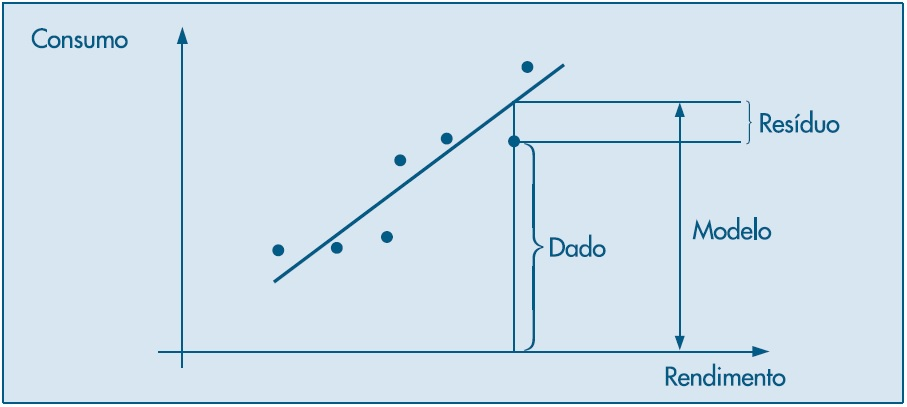
\includegraphics[scale=0.5]{figs/Fig1.jpg}
    \subcaption*{\textbf{Fonte:} \cite{morettin2017estatistica}}
    \label{fig_ex1}
  \end{figure}
\end{frame}

\begin{frame}{}
\frametitle{Modelos}
\begin{block}{}
\justifying
Imagine que estejamos estudando a relação entre rendimentos e gastos de consumo de um conjunto de indivíduos. Podemos obter um gráfico como o da Figura 
\ref{fig_ex1}. O que se espera, intuitivamente, é que os gastos de um indivíduo estejam diretamente relacionados com os seus rendimentos, de modo que é razoável 
supor uma “relação linear” entre essas duas quantidades. Os pontos da Figura \ref{fig_ex1} não estão todos, evidentemente, sobre uma reta, essa seria o nosso padrão 
ou modelo. A diferença entre os dados e o modelo constitui os resíduos.
\end{block}
\end{frame}

\begin{frame}{}
\frametitle{Modelos}
\begin{block}{}
\justifying
De modo esquemático:
\begin{equation}
\label{eq1}
\textrm{Dados}=\textrm{Modelo}\ +\ \textrm{Resíduos,}\quad \textrm{ou, ainda,}\quad 
D=M+R
\end{equation}
\end{block}
\pause
\begin{block}{}
\justifying
A parte M é também chamada parte suave (ou regular ou, ainda, previsível) dos dados, enquanto R é a parte aleatória. 
\end{block}
\pause
\begin{block}{}
\justifying
A parte R é tão importante quanto M, e a análise dos resíduos constitui uma parte fundamental de todo trabalho estatístico. Basicamente, são os resíduos que nos 
dizem se o modelo é adequado ou não para representar os dados.
\end{block}
\end{frame}

\begin{frame}{}
\frametitle{Modelos}
\begin{block}{}
\justifying
Uma análise exploratória de dados busca, essencialmente, fornecer informações
para estabelecer (\ref{eq1}).
\end{block}
\end{frame}

\section{Técnicas Computacionais}
\begin{frame}{}
\frametitle{Técnicas Computacionais}
\begin{block}{}
\justifying
O desenvolvimento rápido e constante na área de computação foi acompanhado pela introdução de novas técnicas de análise de dados, notadamente de métodos 
gráficos e de métodos chamados de computação intensiva.
\end{block}
\end{frame}

\begin{frame}{}
\frametitle{Técnicas Computacionais}
\begin{block}{}
\justifying
Para a implementação dessas técnicas, foram desenvolvidos programas estatísticos, atualmente usados em larga escala tanto no meio acadêmico como em indústrias, 
bancos, órgãos de governo e etc. Um dos mais utilizados na atualidade é o software R.
\end{block}
\begin{figure}[H]
    \centering
    
\includegraphics[height=0.3\textwidth, width=0.8\textwidth]{figs/download.jpg}
    %\caption{Logo R.}
    %\label{fig_ex1}
  \end{figure}
\end{frame}

\begin{frame}{}
\frametitle{Técnicas Computacionais}
\begin{block}{}
\justifying
Por outro lado, os programas podem exigir maior ou menor experiência computacional dos usuários. Alguns operam com menus, e seu uso é mais simples. Outros 
requerem maior familiaridade com o computador e são baseados em linguagens próprias. 
\end{block}
\pause
\begin{block}{}
\justifying
\textbf{Fiquem atentos}, \textbf{procurem aprender programação}, não tenha medo do computador! Estamos a bordo de uma revolução tecnológica que já está transformando 
a forma como vivemos, trabalhamos e nos relacionamos e à medida que todas as empresas se tornam digitais, a demanda por profissionais de tecnologia aumenta 
mais rápido do que a disponibilidade de mão de obra qualificada!
\end{block}
\end{frame}

\begin{frame}{}
\frametitle{Técnicas Computacionais}
\begin{block}{}
\justifying
Além dos pacotes estatísticos, há outros pacotes de grande utilidade para realizar tarefas matemáticas e estatísticas. Dentre estes, mencionamos o Mathematica, o Maple, o Gauss, o Geogebra, o excel e o MatLab. Existe também o Wolfram Alpha e o Symbolab que são mecanismos de conhecimento computacional que funcionam online. Além disso, nesse curso, iremos utilizar o \LaTeX~ como editor de texto.
\end{block}
\begin{figure}[H]
    \centering
    
\includegraphics[height=0.3\textwidth, width=0.8\textwidth]{figs/mylogo.png}
  \end{figure}
\end{frame}

\begin{frame}{}
\frametitle{O Software R}
\begin{block}{}
\justifying
Vamos utilizar no curso, preferencialmente, o software R, que pode ser obtido livremente no Compreensive R Archive Network (CRAN). Como o curso é baseado no livro de Estatística Básica do Pedro Morettin e Wilton Bussab, há um repositório com vários scripts do livro nos endereços: 
\url{www.ime.usp.br/~pam/EstBas.html} e \url{rpubs.com./EstatBasica}.
\end{block}
\end{frame}

\section{Métodos Gráficos}
\begin{frame}{}
\frametitle{Métodos Gráficos}
\begin{block}{}
\justifying
Os métodos gráficos têm encontrado um uso cada vez maior devido ao seu forte apelo visual. Normalmente, é mais fácil para qualquer pessoa entender a mensagem 
de um gráfico do que aquela embutida em tabelas ou sumários numéricos.
\end{block}
\end{frame}

\begin{frame}{}
\frametitle{}
\begin{block}{}
\justifying
Os gráficos são utilizados para:
\begin{itemize}
\item buscar padrões e relações;\pause
\item confirmar (ou não) certas expectativas que se tinha sobre os dados;\pause
\item descobrir novos fenômenos;\pause
\item confirmar (ou não) suposições feitas sobre os procedimentos estatísticos usados; e\pause
\item apresentar resultados de modo mais rápido e fácil.
\end{itemize}
\end{block}
\end{frame}

\begin{frame}{}
\frametitle{}
\begin{block}{}
\justifying
Podemos usar métodos gráficos para plotar os dados originais ou outros dados derivados
deles. Por exemplo, a investigação da relação entre as variáveis da Figura (\ref{fig_ex1}) pode ser feita por meio daquele diagrama de dispersão. Mas podemos também “ajustar” uma reta aos dados, calcular o desvio (resíduo) para cada observação e fazer um novo gráfico, de consumo contra resíduos, para avaliar a qualidade do ajuste.
\end{block}
\end{frame}

\section{Conjuntos de Dados}
\begin{frame}{}
\frametitle{Conjuntos de Dados}
\begin{block}{}
\justifying
Na página da disciplina (\url{https://maf105.github.io/}) aparecem alguns conjuntos de dados que serão utilizados nos exemplos ou nos exercícios propostos. Aconselho a todos a reproduzir os exemplos, usando esses dados, bem como resolver os problemas, pois somente a efetiva manipulação de dados pode levar a um bom entendimento das técnicas apresentadas.
\end{block}
\end{frame}

\begin{frame}{}
\frametitle{}
\begin{block}{}
\justifying
Os conjuntos de dados apresentados provêm de diferentes fontes, que são mencionadas
em cada conjunto e depois explicitadas nas referências. Usaremos para as análises estatísticas o software R, calculadora cientifica e planilhas do Excel. 
\end{block}
\end{frame}

\begin{frame}{}
\frametitle{}
\begin{block}{O novo petróleo!}
\justifying
Em 2006, Clive Robert Humby (Matemático britânico e empresário milionário da área de ciência de dados) cunhou a frase ``Os dados são o novo petróleo'' \cite{Charles}. Michael Palmer expandiu a citação de Humby dizendo, como o petróleo, os dados são ``valiosos, mas se não forem refinados, não podem realmente ser usados. Petróleo deve ser transformado em gás, plástico, produtos químicos, etc. para criar uma entidade valiosa que impulsione atividades lucrativas; então, os dados devem ser desmembrados e analisados para que tenham valor'' \cite{Palmer, Haupt, Firican}.
\end{block}
\end{frame}

\begin{frame}{}
\frametitle{}
\begin{block}{}
\centering
{\Large \bf{Mãos à obra!!!}}
\end{block}
\end{frame}


\begin{frame}[allowframebreaks]
\frametitle{\bf Referências}
\printbibliography
\end{frame}


\end{document}
